\section{Methods}  \label{Methods}

In this section We propose a novel RNN architecture called the Recurrent Perceiver to model an object's changing appearance and motion over time for video object detection.

\subsection{Model}

In the experiment, we augmented the Perceiver architecture \cite{jaeglePerceiverGeneralPerception2021} to support an autoregressive setup. We unroll the model in the time dimension, so the hidden state from the previous frame is propagated to the next frame.

\begin{figure}
    \centering
    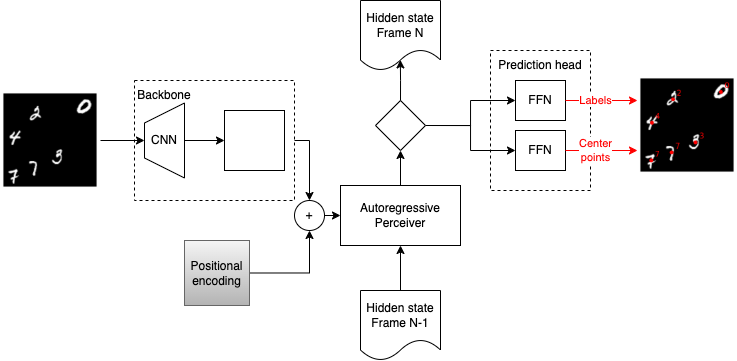
\includegraphics[width=\textwidth]{figures/figure_methods_model_ar_perceiver.png}
    \caption{The autoregressive Perceiver uses a conventional CNN backbone to learn a 2D representation of an input frame. The model flattens it and supplements it with a positional encoding before passing it to the autoregressive Perceiver model. Additionally, the autoregressive Perceiver takes a hidden state from the previous frame. We pass each output embedding of the Perceiver to the feed-forward network (FFN) that predicts class labels and center points.}
    \label{fig:figure_methods_model_ar_perceiver}
\end{figure}

The second variation of the model includes an additional frame view dimension.

\begin{figure}
    \centering
    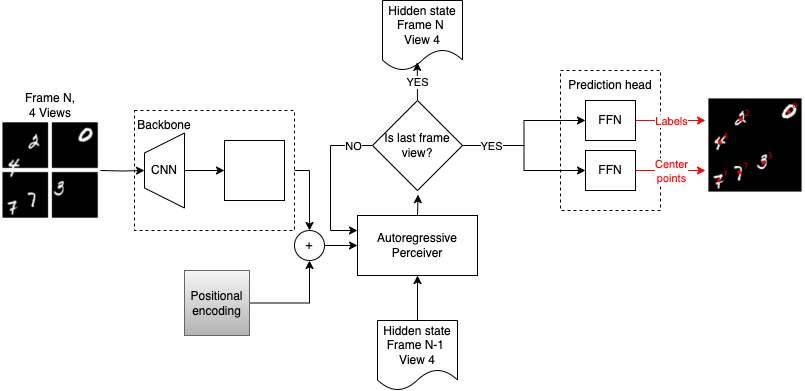
\includegraphics[width=\textwidth]{figures/figure_methods_model_ar_perceiver_views.png}
    \caption{Autoregressive Perceiver with view dimension. The backbone output is supplemented with a learned view-specific positional encoding before passing it to the autoregressive Perceiver model. The autoregressive Perceiver takes a hidden state from the previous frame's last view and iterates through the current frame's views. After the last view, we pass the output embedding of the Perceiver to the feed-forward network (FFN) that predicts class labels and center points on the global frame raster.}
    \label{fig:figure_methods_model_ar_perceiver_views}
\end{figure}


\subsection{Dataset}

For our experiment, we generated our own dataset, which we call "detection-moving-mnist-easy". We took inspiration from the MovingMNIST dataset \cite{srivastava2016unsupervisedlearningvideorepresentations}, which is used for TODO use cases. In our case, we are interested in object detection and tracking tasks.

\begin{figure}
    \centering
    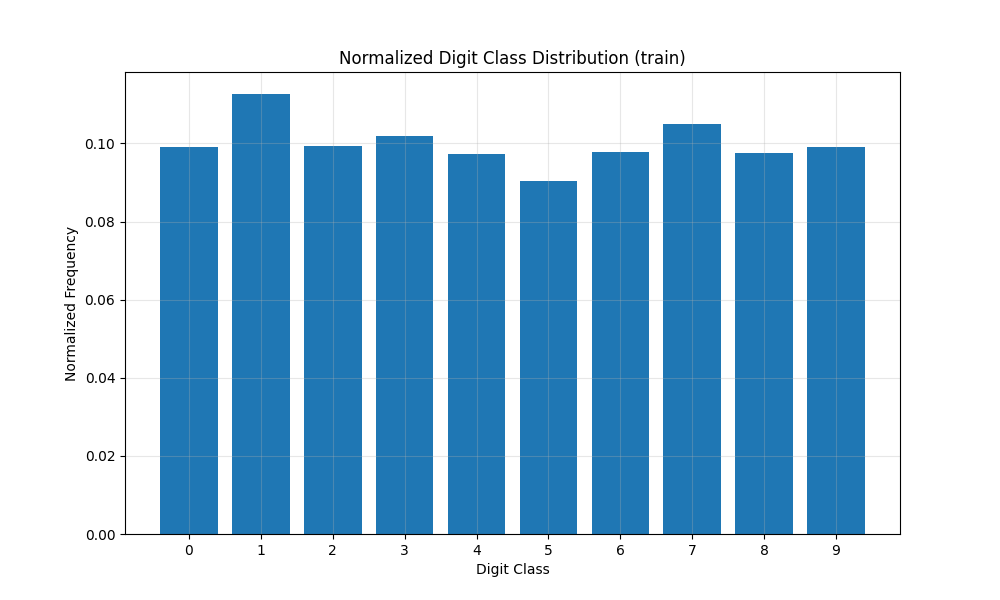
\includegraphics[width=\textwidth]{figures/figure_method_dataset_train_digit_classes.png}
    \caption{Distribution of classes in the "detection-moving-mnist-easy" dataset.}
    \label{fig:figure_method_dataset_train_digit_classes}
\end{figure}

We hosted the dataset on Hugging Face \footnote{\url{https://huggingface.co/datasets/Max-Ploter/detection-moving-mnist-easy}}. For the first frame, we pick a number of digits from 1 to 10 with uniform probability (see Figure~\ref{fig:figure_method_dataset_train_digit_classes}). Depending on the number of digits per first frame, we draw, without replacement, from the well-known MNIST dataset (from the train and test splits corresponding to the dataset split). To each digit, we assign an affine translation from -5 to 5 randomly with uniform probability. Also, there is an additional greedy algorithm that places digits on the first frame randomly and tries to avoid overlaps. Then, we apply corresponding affine transformations to move the digits through 20 frames on the canvas image of size 128x128. As a result, we receive a tensor of size 20x1x128x128, which represents a video (see Figure~\ref{fig:figure_methods_dataset_detection_mmnist_sequence}).


\begin{figure}
    \centering
    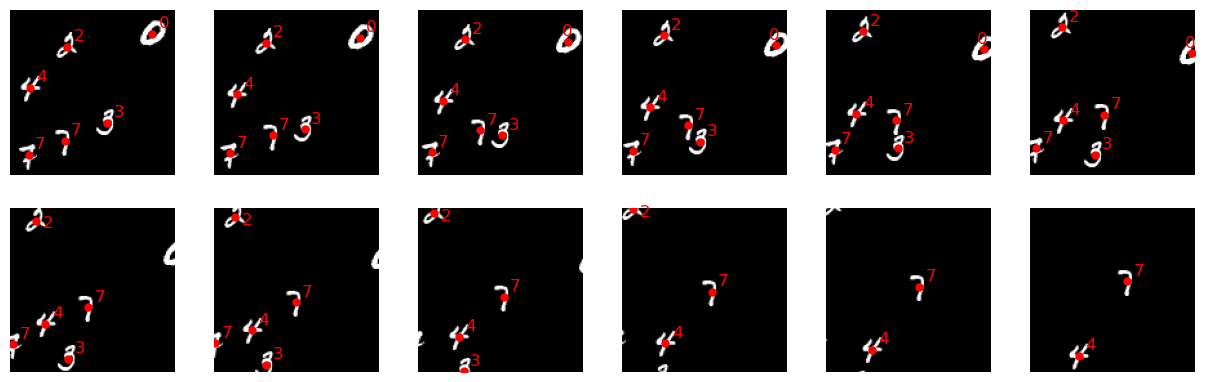
\includegraphics[width=\textwidth]{figures/figure_methods_dataset_detection_mmnist_sequence.png}
    \caption{Example of 12 frames from the sequence. Ground truth, shown in red, indicates the ground truth digit center point and a class label.}
    \label{fig:figure_methods_dataset_detection_mmnist_sequence}
\end{figure}



We do not restrict digit overlap in subsequent frames. It is even possible to have some degree of overlap in the first frame if the greedy algorithm is unable to randomly place digits in such a way on the first frame.
We do not bounce digits against image boundaries, so each digit can leave the frame. You can see in the figure that later frames have fewer digits (see Figure~\ref{fig:figure_method_dataset_train_digits_per_frame}).

% TODO DOUBLE CHECK number this plot
\begin{figure}
    \centering
    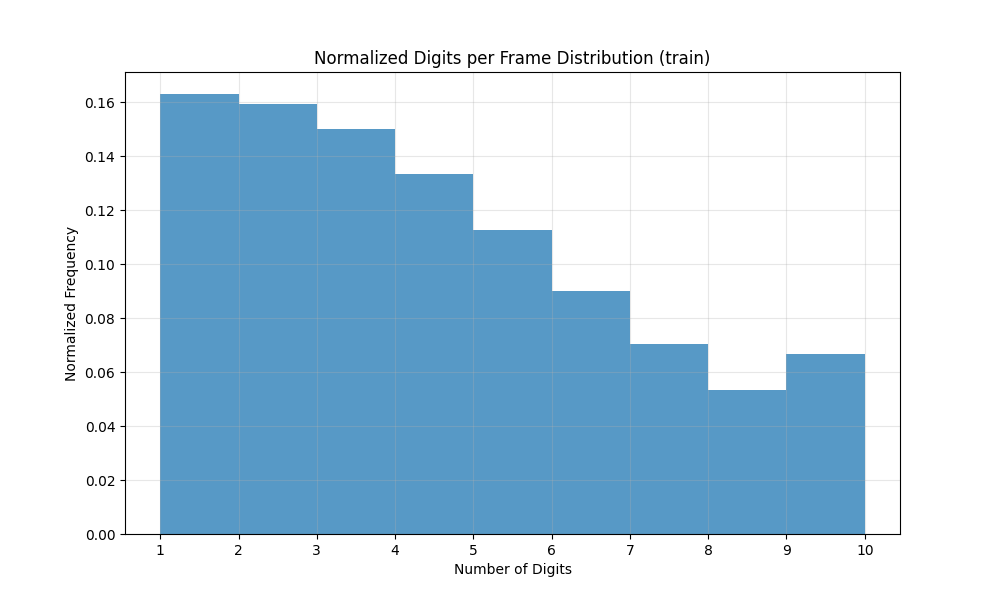
\includegraphics[width=\textwidth]{figures/figure_method_dataset_train_digits_per_frame.png}
    \caption{Distribution of classes in the "detection-moving-mnist-easy" dataset.}
    \label{fig:figure_method_dataset_train_digits_per_frame}
\end{figure}


We generated the dataset with 60K and 10K train and test splits, respectively.

Annotations, automatically generated during sequence creation, include digit classes and digit center point coordinates, with the coordinate system in the center of the image.

For the purpose of some of the experiment we additionally divide the frame into grid views. In this way we mimic a Bird Eye View (BEV) (see Figure~\ref{fig:figure_methods_dataset_image_view_bev}).

\begin{figure}
    \centering
    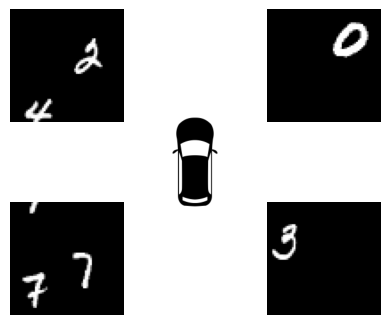
\includegraphics[width=0.33\textwidth]{figures/figure_methods_dataset_image_view_bev.png}
    \caption{Bird Eye View (BEV) of the frame raster divided into grid.}
    \label{fig:figure_methods_dataset_image_view_bev}
\end{figure}


\subsection{Training Procedures} \label{TrainingProcedures}

We implemented two training procedures: \texttt{shuffle} and \texttt{dropout}. Additionally, we implemented a combination of the two. A model trained without applying these training procedures is considered the baseline.

\begin{description}
    \item[\texttt{shuffle}] In this procedure, the sensor inputs are randomly permuted within each time step. Consequently, the model receives inputs from the sensors in a random order for that specific time step. This shuffling only occurs for sensor inputs within the same time step. This training procedure is only applicable to a multi-view setup.

    \item[\texttt{dropout}] This procedure simulates scenarios where sensor information is missing. To achieve this, we train the model by intermittently dropping sensor inputs (input dropout). We keep the first half of the input sequence intact (no dropout), allowing the model to accumulate features in its hidden state. The second half of the sequence may undergo frame dropout. During training, we gradually increase the probability of an information drop from 10\% to approximately 90\%, with the final value depending on the specific experiment.
\end{description}



% TODO add schema of shuffle and dropout

% TASK DEFINITION

% METRICS